\documentclass[final]{beamer}

\usepackage[orientation=portrait,size=a3,scale=1.0]{beamerposter}

\usepackage[utf8]{inputenc}
\usepackage[T1]{fontenc}
\usepackage{helvet}
\renewcommand{\familydefault}{\sfdefault}
\usepackage{tcolorbox}
\usepackage{tikz}
\usepackage{booktabs}
\usepackage{array}
\usepackage{xcolor}
\usepackage{microtype}
\usepackage{enumitem}
\usepackage{tabularx}
\usepackage{amsmath}
\usepackage{graphicx}

\tcbuselibrary{skins, breakable}

\definecolor{hogentred}{RGB}{178,51,47}
\definecolor{hogentdark}{RGB}{26,26,26}
\definecolor{hogentcream}{RGB}{242,235,231}
\definecolor{hogentmuted}{RGB}{107,95,88}
\definecolor{hogentcream2}{RGB}{233,223,216}
\definecolor{scengreen}{RGB}{46,125,79}
\definecolor{scenyellow}{RGB}{180,130,30}

\setbeamertemplate{navigation symbols}{}
\setbeamercolor{background canvas}{bg=hogentcream}

\tcbset{
    postercard/.style={
        colback=white, colframe=white, arc=3mm, boxrule=0pt,
        drop shadow={opacity=0.10, shadow xshift=0.4mm, shadow yshift=-0.4mm},
        left=5mm, right=5mm, top=4mm, bottom=4mm,
    },
    redcard/.style={
        colback=hogentred, colframe=hogentred,
        colupper=white, arc=3mm, boxrule=0pt,
        left=5mm, right=5mm, top=5mm, bottom=5mm,
    },
    darkcard/.style={
        colback=hogentdark, colframe=hogentdark,
        colupper=hogentcream, arc=3mm, boxrule=0pt,
        left=5mm, right=5mm, top=4mm, bottom=4mm,
    },
    subqbox/.style={
        colback=hogentcream2, colframe=hogentcream2,
        arc=2mm, boxrule=0pt,
        left=3mm, right=3mm, top=2mm, bottom=2mm,
    },
}

\newcommand{\seclabel}[1]{%
    \begin{tikzpicture}[baseline=-0.5ex]
        \node[fill=hogentred, text=white, rounded corners=1.8mm,
        font=\LARGE\bfseries, inner sep=2.2mm,
        minimum width=10mm, minimum height=10mm] {#1};
\end{tikzpicture}}

\newcommand{\secheading}[2]{%
    \noindent\seclabel{#1}\hspace{3mm}%
    {\LARGE\bfseries #2}\par\vspace{2.5mm}}

\newcommand{\secheadingdark}[2]{%
    \noindent\seclabel{#1}\hspace{3mm}%
    {\LARGE\bfseries\color{hogentcream} #2}\par\vspace{2.5mm}}

\newlist{arrowlist}{itemize}{1}
\setlist[arrowlist]{label={\color{hogentred}$\rightarrow$},
    leftmargin=7mm, itemsep=2mm, topsep=1.5mm}

\newlist{dotlist}{itemize}{1}
\setlist[dotlist]{label={\color{hogentred}\textbullet},
    leftmargin=5mm, itemsep=1mm, topsep=0.5mm, parsep=0pt}

\newcommand{\stepnode}[2]{%
    \noindent
    \begin{tikzpicture}[baseline=(n.base)]
        \node[circle, fill=hogentdark, text=white, font=\normalsize\bfseries,
        inner sep=1.8mm, minimum size=8mm] (n) {#1};
    \end{tikzpicture}%
    \hspace{2.5mm}{\normalsize\textbf{\color{hogentred}#2}}%
}

\newcommand{\metricbox}[2]{%
    \begin{tcolorbox}[colback=white,colframe=white,arc=2mm,boxrule=0pt,
        drop shadow={opacity=0.08},
        halign=center,left=1mm,right=1mm,top=1.5mm,bottom=1.5mm]
        {\huge\bfseries\color{hogentred} #1}\par\vspace{0.5mm}
        {\scriptsize\color{hogentmuted} #2}
\end{tcolorbox}}

\newcommand{\scenbar}[4]{%
    \noindent
    \begin{tabularx}{\linewidth}{p{22mm}X}
        \begin{minipage}[c]{22mm}
            {\small\bfseries #1}\\[-0.3mm]{\footnotesize\color{hogentmuted}#2}
        \end{minipage} &
        \colorbox{#3}{%
            \begin{minipage}[c][6.5mm]{\linewidth}%
                \small\bfseries\color{white}\hspace{1.5mm}#4%
        \end{minipage}}
    \end{tabularx}\par\vspace{2mm}}

\begin{document}
    \begin{frame}[t]{}
        
        \begin{tikzpicture}[remember picture,overlay]
            \fill[hogentdark]
            (current page.north west) rectangle ([yshift=-46mm]current page.north east);
            \fill[hogentred]
            ([yshift=-46mm]current page.north west) rectangle
            ([yshift=-49mm]current page.north east);
        \end{tikzpicture}
        
        \vspace{1mm}
        \begin{columns}[T]
            \column{0.65\linewidth}
            {\fontsize{9}{11}\selectfont\bfseries\color{hogentred}%
                \MakeUppercase{Bachelorproef Toegepaste Informatica%
                    ~\textbullet~HOGENT 2025--2026~\textbullet~Software Development}}
            \par\vspace{2mm}
            {\fontsize{32}{34}\selectfont\bfseries\color{white}%
                Augmented Reality op het \textit{\color{hogentred}kerkhof}}
            \par\vspace{2mm}
            \column{0.35\linewidth}
            \raggedleft
            {\normalsize\color{hogentcream!70!hogentdark}%
                Promotor: Dhr.\ S.\ Van Impe\\
                Co-promotor: Dhr.\ L.\ Gvasalia\\[1mm]
                Casus: gem.\ kerkhof Sint-Gillis-Waas}
        \end{columns}
        \vspace{2mm}
        {\large\color{white}\textbf{\color{hogentred}Jens}~Meersschaert}
        \vspace{10mm}
        
        \begin{columns}[T, totalwidth=\linewidth]
            
            \column{0.565\linewidth}
            
            \begin{tcolorbox}[postercard]
                \secheading{1}{Het probleem}
                {\normalsize Een bezoek aan een begraafplaats is een emotioneel moment van
                    herdenking. Toch wordt dat moment vaak verstoord doordat bezoekers het graf
                    van een dierbare niet terugvinden, een tijdrovende en stressvolle ervaring
                    op grote of uniform ingedeelde begraafplaatsen \mbox{(H\"akkil\"a et al., 2022).}}
                
                \vspace{2.5mm}
                \begin{tcolorbox}[colback=hogentcream2, colframe=hogentcream2, arc=2mm,
                    boxrule=0pt, left=4mm, right=4mm, top=2mm, bottom=2mm,
                    borderline west={1.4mm}{0pt}{hogentred}]
                    {\normalsize\itshape\color{hogentred!80!black}%
                        ''Ik stond er gewoon naast. Ik keek er overheen. Het was even verwarrend.''}
                    \\[1.5mm]
                    {\small\color{hogentmuted}%
                        --- Bezoeker, natuurbegraafplaats Hillig Meer (Meer, 2025)}
                \end{tcolorbox}
                
                \vspace{2.5mm}
                {\normalsize Het probleem is leeftijdsonafhankelijk: in de test vond
                    \textbf{geen enkele} testpersoon het graf zonder hulp (Scenario A).
                    Beide werden gefrustreerd na zoeken op jaartal en alfabet zonder resultaat.}
            \end{tcolorbox}
            
            \vspace{2mm}
            
            \begin{tcolorbox}[redcard]
                {\small\bfseries\color{white!60!hogentred}%
                    \MakeUppercase{Onderzoeksvraag}}
                \par\vspace{2.5mm}
                {\large\bfseries\itshape
                    Op welke manier kan digitalisatie, in combinatie met Augmented Reality,
                    worden ingezet om de efficientie van het navigeren op een kerkhof te
                    verbeteren?}
            \end{tcolorbox}
            
            \vspace{2mm}
            
            \begin{columns}[T, totalwidth=\linewidth]
                \column{0.333\linewidth}
                \begin{tcolorbox}[subqbox]
                    {\small\bfseries\color{hogentred}\MakeUppercase{Gebruiker}}\\[1.5mm]
                    \begin{dotlist}
                        \item[\small\color{hogentred}\textbullet] {\small Moeilijkheden bezoekers?}
                        \item[\small\color{hogentred}\textbullet] {\small Behoeften per leeftijd?}
                        \item[\small\color{hogentred}\textbullet] {\small Rust \& sereniteit?}
                    \end{dotlist}
                \end{tcolorbox}
                \column{0.333\linewidth}
                \begin{tcolorbox}[subqbox]
                    {\small\bfseries\color{hogentred}\MakeUppercase{Technologie}}\\[1.5mm]
                    \begin{dotlist}
                        \item[\small\color{hogentred}\textbullet] {\small Beperkingen tools?}
                        \item[\small\color{hogentred}\textbullet] {\small Hoe kan AR helpen?}
                        \item[\small\color{hogentred}\textbullet] {\small AR + kaart samen?}
                    \end{dotlist}
                \end{tcolorbox}
                \column{0.333\linewidth}
                \begin{tcolorbox}[subqbox]
                    {\small\bfseries\color{hogentred}\MakeUppercase{Data \& Recht}}\\[1.5mm]
                    \begin{dotlist}
                        \item[\small\color{hogentred}\textbullet] {\small Privacygevoelig?}
                        \item[\small\color{hogentred}\textbullet] {\small Wat veilig te gebruiken?}
                        \item[\small\color{hogentred}\textbullet] {\small GDPR-implicaties?}
                    \end{dotlist}
                \end{tcolorbox}
            \end{columns}
            
            \vspace{2mm}
            
            \begin{tcolorbox}[postercard]
                \secheading{2}{Wat bestaat er al? Wat mist er?}
                {\normalsize Digitalisatie van begraafplaatsen helpt aantoonbaar: bezoekers
                    vinden graven sneller terug na invoering van een digitale tool
                    (H\"akkil\"a et al., 2022). Toch missen er nog dingen:}
                \vspace{2mm}
                \begin{arrowlist}
                    \item {\normalsize\textbf{Geoloket (Beveren, Cevi)}: publieke
                        kaarttool, maar de blik moet voortdurend wisselen tussen scherm en
                        omgeving, wat de cognitieve belasting verhoogt (Zhao et al., 2025)}
                    \item {\normalsize\textbf{WebBGP (Sint-Gillis-Waas, Cevi)}: bevat
                        alle grafdata, maar is \emph{enkel intern} en biedt geen hulp aan
                        bezoekers (Lesdanon, persoonlijk interview, 2025)}
                    \item {\normalsize\textbf{Drempel voor ouderen}: kaartinterfaces worden
                        door minder tech-vaardige bezoekers als weinig intu{\"i}tief ervaren
                        (H\"akkil\"a et al., 2022)}
                \end{arrowlist}
                \vspace{2mm}
                \begin{tcolorbox}[colback=hogentcream2, colframe=hogentcream2, arc=2mm,
                    boxrule=0pt, left=4mm, right=4mm, top=2mm, bottom=2mm,
                    borderline west={1.4mm}{0pt}{hogentred}]
{\normalsize\textbf{\color{hogentred}Wat ontbreekt:} bestaande oplossingen tonen
    de weg op een kaart, maar kijken doet de bezoeker nog altijd zelf.
    AR projecteert navigatie rechtstreeks in het zichtveld en elimineert
    die cognitieve wissel (Zhao et al., 2025; Xu, 2018).}
                \end{tcolorbox}
            \end{tcolorbox}
            
            \vspace{2mm}
            
            \begin{tcolorbox}[postercard]
                \secheading{3}{Methode}
                \vspace{1.5mm}
                \stepnode{1}{Voorbereiding}~{\normalsize--- risicoanalyse, interview gemeente (WebBGP), terreinanalyse}\\[3mm]
                \stepnode{2}{Ontwerp}~{\normalsize--- gelaagde architectuur, gebruikersflow, AR-logica}\\[3mm]
                \stepnode{3}{Juridische analyse}~{\normalsize--- GDPR, rijksregisternummer, verwerkersovereenkomst}\\[3mm]
                \stepnode{4}{Implementatie}~{\normalsize--- Swift \& ARKit, iteraties op fysiek toestel}\\[3mm]
                \stepnode{5}{Testen}~{\normalsize--- 3 scenario's (A/B/C), 3 testpersonen op locatie}\\[3mm]
                \stepnode{6}{Evaluatie}~{\normalsize--- onderzoeksvragen beantwoord, aanbevelingen}
            \end{tcolorbox}
            
            \vspace{2mm}
            
            \begin{tcolorbox}[colback=hogentcream2, colframe=hogentcream2, arc=2mm,
                boxrule=0pt, left=4mm, right=4mm, top=2.5mm, bottom=2.5mm]
                {\small\bfseries\color{hogentred}\MakeUppercase{Bronnen}}
                \par\vspace{1.5mm}
                {\footnotesize\color{hogentmuted}%
                    H\"akkil\"a, J., et al.\ (2022). \textit{Exploring pervasive displays for cemeteries
                        and memorial sites.} Personal and Ubiquitous Computing, 26(3), 737--747.
                    ~$\bullet$~
                    Zhao, Y., et al.\ (2025). \textit{A Systematic Review of the Use of Augmented
                        Reality in Pedestrian Navigation.} ACM Computing Surveys, 58(5), 1--32.
                    ~$\bullet$~
                    Xu, Y.\ (2018). \textit{Exploring the benefits and challenges of AR in an outdoor
                        tourism experience.}
                    ~$\bullet$~
                    Novack, T., et al.\ (2018). \textit{A System for Generating Customized Pleasant
                        Pedestrian Routes Based on OpenStreetMap Data.} Sensors.
                    ~$\bullet$~
                    Meer, H.\ (2025). \textit{Een graf terugvinden op Hillig Meer.}
                    ~$\bullet$~
                    LLC, G.\ (2025). \textit{ARCore: Google's platform for augmented reality.}
                    ~$\bullet$~
                    Wet van 8 augustus 1983 tot regeling van een Rijksregister van de natuurlijke
                    personen.
                    ~$\bullet$~
                    GDPR (2016/679), overweging 27 --- niet van toepassing op gegevens van
                    overledenen.}
            \end{tcolorbox}
            
            \column{0.02\linewidth}
            \column{0.415\linewidth}
            
            \begin{tcolorbox}[postercard]
                \secheading{4}{Oplossing: de POC}
                \begin{columns}[T, totalwidth=\linewidth]
                    \column{0.52\linewidth}
                    {\normalsize Een iOS proof of concept (Swift $\cdot$ ARKit $\cdot$ SceneKit)
                        die de kaart niet vervangt maar \textbf{aanvult} met AR:}
                    \vspace{2mm}
                    \begin{arrowlist}
                        \item {\normalsize\textbf{3D AR-navigatiepijl}: blik blijft op de omgeving}
                        \item {\normalsize\textbf{World-locked grafmarker}: lichtbalk van 6\,m zichtbaar over meerdere rijen}
                        \item {\normalsize\textbf{Satellietminikaart}: overzicht \& fallback}
                    \end{arrowlist}
                    \vspace{2mm}
                    {\small\color{hogentmuted}GPS$\rightarrow$AR via vlakke-Aarde-benadering
                        (fout $<$0,01\%, Xu, 2018) $\cdot$ overdraagbaar naar Android via ARCore (LLC, 2025).}
                    \column{0.04\linewidth}
                    \column{0.44\linewidth}
                    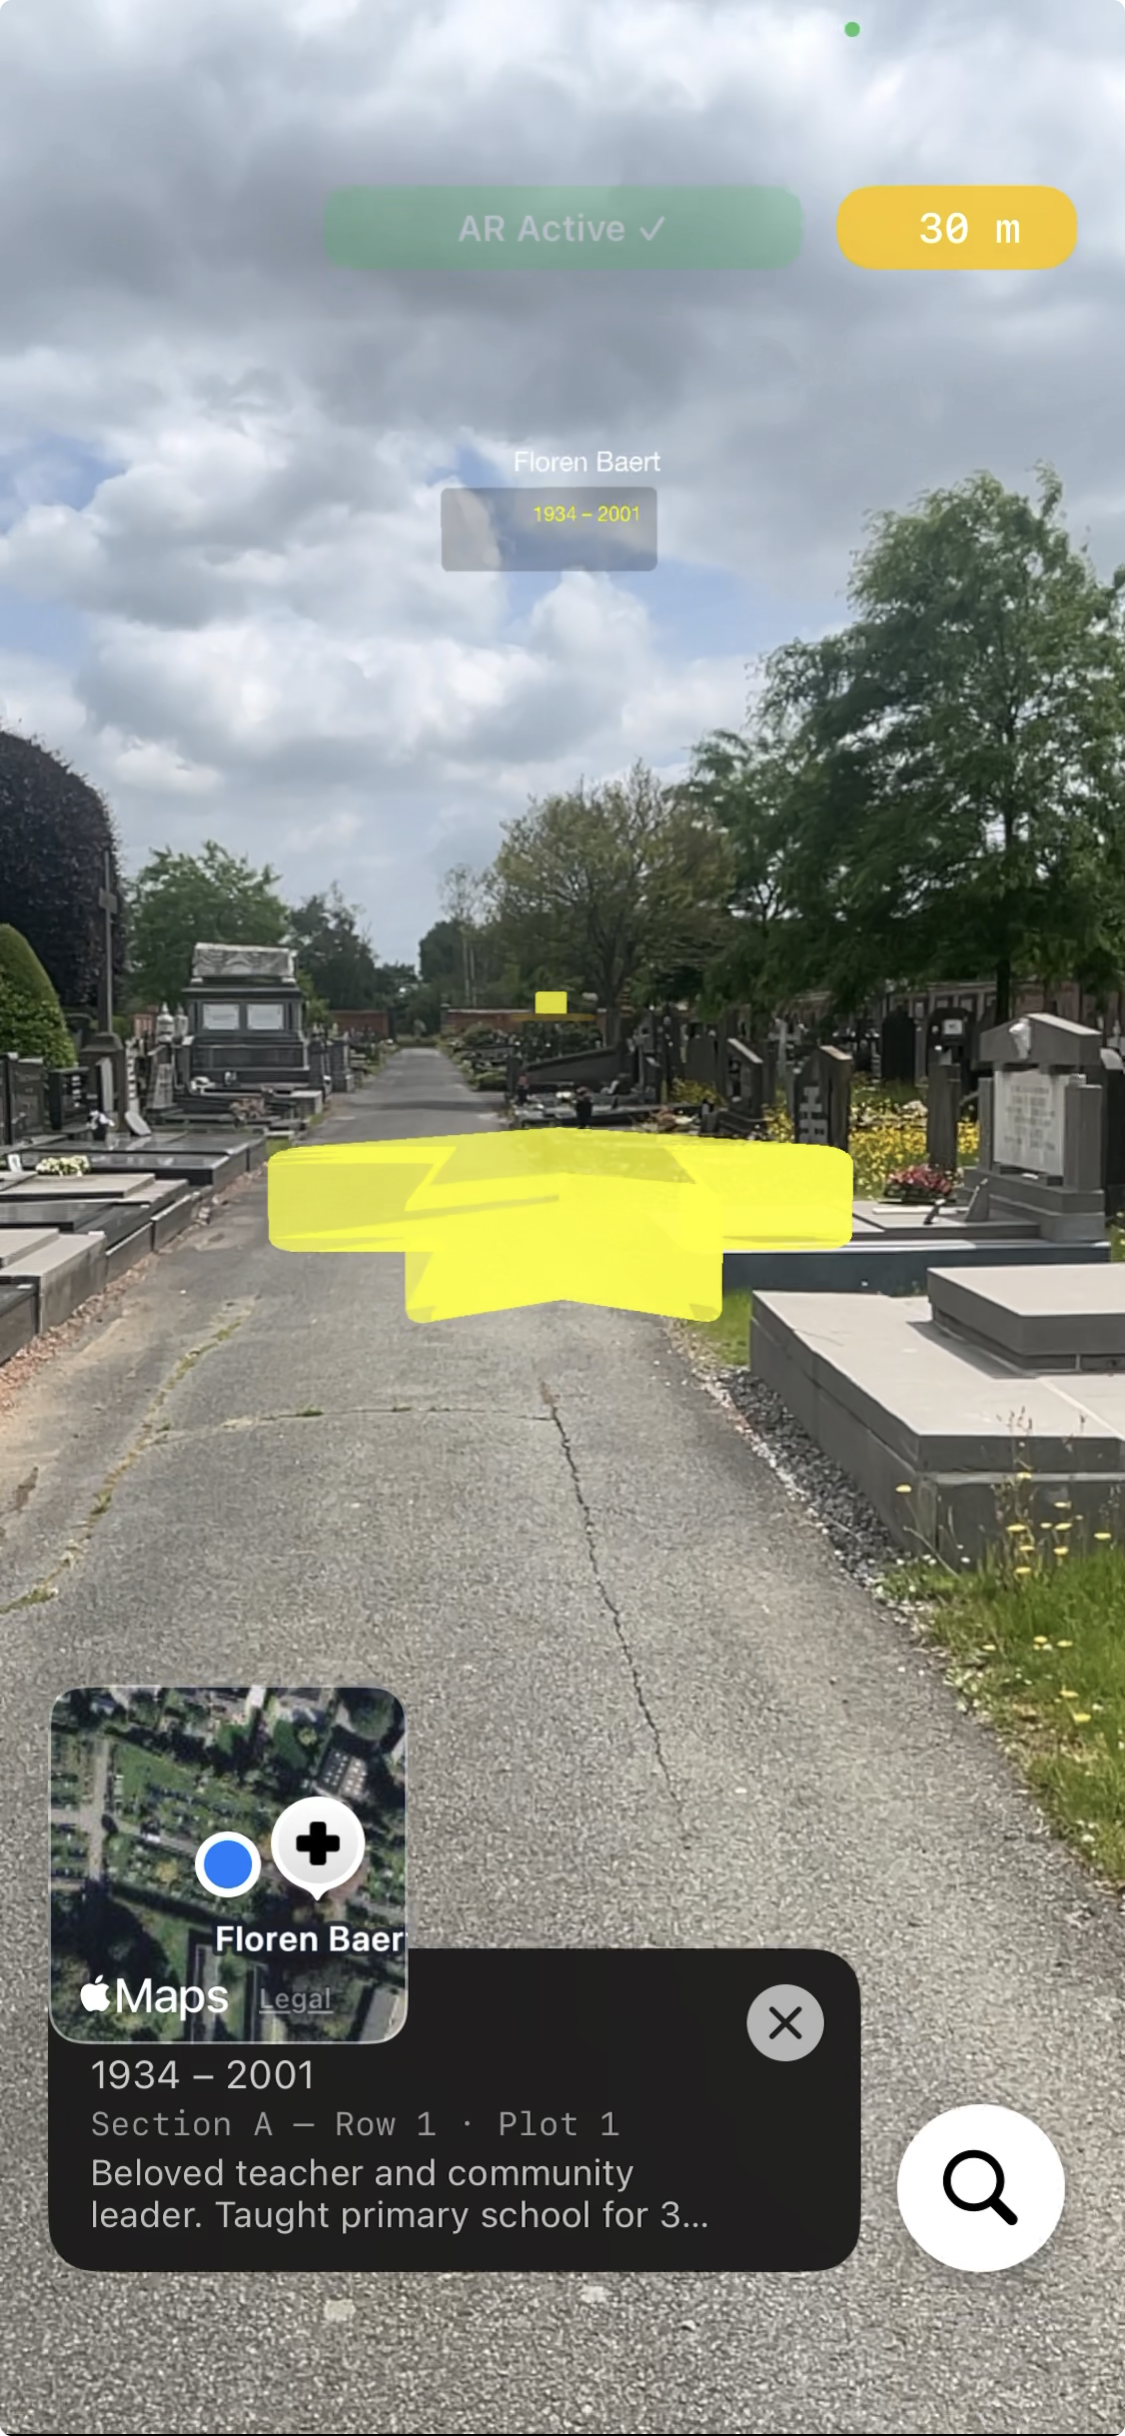
\includegraphics[width=\linewidth]{graphics/poc-ss.png}
                \end{columns}
            \end{tcolorbox}
            
            \vspace{2mm}
            
            \begin{tcolorbox}[postercard]
                \secheading{5}{Resultaten}
                {\normalsize Drie scenario's, twee externe testpersonen, kerkhof
                    Sint-Gillis-Waas:}
                \vspace{2.5mm}
                
                \scenbar{Scenario A}{Geen hulp}{hogentred}{Graf \textbf{niet gevonden}}
                \scenbar{Scenario B}{Enkel kaart}{scenyellow}{Gevonden~$\cdot$~routelijn \textbf{gemist}}
                \scenbar{Scenario C}{Volledige AR}{scengreen}{Snelst \& meest intuïtief}
                
                \vspace{3mm}
                \begin{columns}[T, totalwidth=\linewidth]
                    \column{0.33\linewidth}\metricbox{2'35''}{snelste tijd (AR)}
                    \column{0.33\linewidth}\metricbox{7--8\,/\,10}{subjectief oordeel}
                    \column{0.33\linewidth}\metricbox{0\,/\,2}{zonder app}
                \end{columns}
                
                \vspace{2.5mm}
                {\normalsize\textbf{Verbeterpunten uit de tests:}}
                \begin{arrowlist}
                    \item {\normalsize\textbf{Onboarding}: TP3 (49 j.) ontdekte de AR-overlay
                        pas na een tip; beide vroegen om een introductiemelding}
                    \item {\normalsize\textbf{Routelijn}: beide verwachtten een padgewijze
                        lijn, vereist GIS-paddata (Novack et al., 2018)}
                \end{arrowlist}
            \end{tcolorbox}
            
            \vspace{2mm}
            
            \begin{tcolorbox}[postercard]
                \secheading{\S}{Privacy \& recht}
                \begin{arrowlist}
                    \item {\normalsize Grafdata van overledenen valt \textbf{buiten de GDPR}
                        (overweging 27), maar vraagt zorgvuldigheid wegens indirecte link met
                        nabestaanden}
                    \item {\normalsize Rijksregisternummer \textbf{categorisch verboden}
                        (Wet 8 aug.\ 1983)}
                    \item {\normalsize Productie vereist verwerkersovereenkomst,
                        privacyverklaring en mogelijk een DPIA}
                \end{arrowlist}
            \end{tcolorbox}
            
            \vspace{0.5mm}
            
            \begin{tcolorbox}[darkcard]
                \secheadingdark{C}{Conclusie}
                {\large\bfseries\itshape\color{hogentcream}%
                    AR werkt voor kerkhofnavigatie, 
                    \textbf{\color{hogentred!60!white}maar enkel in combinatie met een kaart.}}
                \vspace{2.5mm}
                \begin{arrowlist}
                    \item {\normalsize\color{hogentcream!90!white}
                        \textbf{Hybride model}: AR-pijl + minikaart vullen elkaar aan}
                    \item {\normalsize\color{hogentcream!90!white}
                        \textbf{Technisch haalbaar} en platformonafhankelijk}
                    \item {\normalsize\color{hogentcream!90!white}
                        \textbf{Eerste bouwsteen} voor een gemeentelijke productie-app mits
                        GIS-data en juridische afspraken}
                \end{arrowlist}
            \end{tcolorbox}
            
        \end{columns}
        
        \vspace{2mm}
        

        \noindent
        {\small\color{hogentmuted}%
            Proof of Concept~$\cdot$~\textbf{iOS~$\cdot$~Swift~$\cdot$~ARKit~$\cdot$~SceneKit}%
            \hfill
            \textbf{\color{hogentred}\#AugmentedReality}~~%
            \textbf{\color{hogentred}\#Kerkhofnavigatie}~~%
            \textbf{\color{hogentred}\#ARKit}~~%
            \textbf{\color{hogentred}\#GDPR}}
        
    \end{frame}
\end{document}